\nomenclature[]{VRP}{Vehicle Routing Problem}

\section{Scene Surveying}\label{sec:SceneSurveying}
This section outlines the algorithms that were explored to generate a set of routes for the RAVs that will be used to record sensor data at each of the grid points generated in the region of interest. We gave a high-level description of this problem at the beginning of Chapter \ref{chapter:SceneSurveying}:
"\textit{Find a set of routes for each of $K$ RAVs to be used in the data-gathering process, such that these sets partition $R$ and the cost of the system of RAVs traversing these points is minimized}".
%which are generated using Algorithm \ref{alg:GridGeneration} described in the preceding section. 
We make some assumptions related to the solution of this problem:
\note{This list might not cover everything, come back to it}
\begin{itemize}
    \item Each RAV is assumed to have the same internal representation of the region of interest, namely the set of uniformly spaced grid points generated by Algorithm \ref{alg:GridGeneration}.
    \item Each RAV is assumed to have the ability to move between any pair of grid points unobstructed using the shortest possible path.
    \item RAVs are assumed to move with a fixed operational velocity, which can vary between RAVs.
    \item Each RAV may be equipped with different sensors to the others and it is assumed that sensing times may vary among the RAVs.
    \item Each RAV has a finite battery capacity which implies they have a finite amount of time that they can fly for before they need to recharge.
\end{itemize}

%Talk about how problem was transformed to TSP problem, took that and then divided up soln for mTSP.

The scene surveying problem that we would like to solve can be treated as an instance of the \textit{Vehicle Routing Problem} (VRP), which was first described in a paper by \citeauthor{Dantzig1959TheProblem} \cite{Dantzig1959TheProblem}. This problem is a generalisation of the classic \textit{Travelling Salesman problem} (TSP). There are many variants and extensions to this problem, but the VRP essentially asks for a set of routes to be assigned to the RAVs such that each point in the graph is visited exactly once, which minimises the total time taken to "service" each of the points \cite{Dantzig1959TheProblem}. In our case, the service time is the time taken to record a sensor reading. We are interested in solving this problem where the graph is defined by the grid of points that is generated using Algorithm \ref{alg:GridGeneration}. A formal definition of the VRP and its variants can be found in \cite{Toth2002TheProblem}.

\subsection{Simplified Problem}\label{subsec:SimplifiedVRP}
\note{maybe change this to constrained problem or something similar}
We began by taking a simplified version of the full vehicle routing problem in order to explore possible solutions. This section expands on our published work in \cite{Smyth2018UsingDrones}, which summarises how this simplified problem was tackled. Rather than concern ourselves with the details of sensor sampling times and battery constraints, we first focused on designing a solution that can assign a set of routes to a homogeneous set of RAVs. 
%We assumed that service times add a fixed constant to the total time taken to perform the survey (and can hence be ignored) and we ignore the time added that the RAVs might need to recharge. 
The problem can be described as follows:
\\
\textit{Given a fully connected graph, $G$, to visit and $n$ RAV agents, find a subtour for each agent such that each point in $P \in G$ is visited exactly once by any agent in the system, with the objective of minimizing the longest time taken for any individual agent subtour, in order to minimize the time taken to carry out the survey.}
\\
This is the \textit{multiple Travelling Salesman Problem} (mTSP). 

%According to the number of distribution centers: single distribution center and multi-distribution center problem;
%According to the type of vehicle: single-vehicle type and multi-vehicle type problem;
%According to the characteristics of the task: pure send (take) cargo problems and loading and unloading mixing problem;
%According to whether the time constraints: no time window problem and time window problem;
%By vehicle loading: And the problem of non-full load;
%According to the optimization of the number of goals: a single objective and multi-objective problem;
%Vehicle and vehicle by the ownership of the points: the vehicle open problem and vehicle closure problems;
%By mastering the information of certainty: Sexual VRP and non-deterministic VRP problems;
%As can be seen from these classifications, solutions to the VRP problem are varied, each category 

\subsection{Proposed Solution for the Simplified Problem}
\note{Again maybe use constrained instead of simplified}
Due to the fact that the mTSP is at least as hard as the TSP, since it is a generalisation of the TSP, finding a polynomial time solution to the mTSP is not feasible. We explored a number of sub-optimal solutions that take advantage of the highly structured nature of the uniformly spaced grid that we use in our instance of the problem. The usual trade-off between solution quality vs. time taken to find the solution motivated our choice of implemented algorithm, as we anticipated that the time taken to execute the planned routes may be comparable to the time taken to generate some solutions (the order of minutes or hours). For example, \citeauthor{Hungerlander2018TheGrids} shows the results of using a Mixed Integer Linear Program (MILP) took hours to run for grid sizes that could be considered relatively small in many real-world domains \cite{Hungerlander2018TheGrids}.
%which would exceed the amount of time taken to perform even a random solution. %General details of solutions that can be applied to solve the mTSP and VRP can be found in Section <> of the literature review (this will be filled in).

\subsubsection{Nearest Neighbor Algorithm}
There are four common heuristic algorithms that form the basis of most solutions to TSP and mTSP problems, as stated in \cite{Johnson1997TheOptimization}: the \textit{nearest neighbor} algorithm, the \textit{greedy algorithm}, the \textit{Clarke-Wright} algorithm and the \textit{Christofides} algorithm. We began by implementing an algorithm which is a modification of a TSP solution based on the nearest-neighbor heuristic. Our reasoning is based on the following premises:
\begin{enumerate}
    \item The nearest-neighbor heuristic is a well-known heuristic that is straightforward to implement. It is known to provide good results to the TSP when the cost is defined as the Euclidean distance between points \cite{Johnson1995TheOptimization}, as in our use case.
    \item The nearest-neighbor solution to the TSP can be very easily modified to be applied to the mTSP by implementing it in a round-robin manner, as detailed in Algorithm \ref{alg:NNHeuristic}.
    \item The nearest-neighbor heuristic is known to have a running time which is O($n^2$) \cite{Rosenkrantz1977AnProblem}, which means it can scale well to reasonably large problem instances compared to other algorithms which have a far worse performance complexity. For example, the Christofides algorithm is known to be within a factor of $\frac{3}{2}$ of the optimal solution, but its running time is O($n^3$) \cite{Christofides1976WORST-CASEPROBLEM}, which quickly becomes prohibitively long.
    %\item Partitioning a TSP solution can give very good mTSP solutions on the same graph.
\end{enumerate}

The nearest-neighbor (NN) heuristic algorithm for the multiple Travelling Salesman problem is shown in Algorithm \ref{alg:NNHeuristic}.


\begin{algorithm}[h]
\caption{The Nearest-Neighbor Solution to the mTSP Problem}
\label{alg:NNHeuristic}
\begin{algorithmic}[1]
\renewcommand{\algorithmicrequire}{\textbf{Input:}}
\renewcommand{\algorithmicensure}{\textbf{Output:}}

\REQUIRE$ \newline k \quad \text{ The number of RAVs in the mTSP }
\newline way\_points \quad \text{ The set of points the RAVs must visit }
\newline cost(i,j) \quad \text{ The function giving the cost of travelling from node i to node j }
$
\ENSURE $ \newline RAV\_routes \quad \text{A key-value data structure mapping RAVs to their corresponding routes.}
$

\hfill\pagebreak

%\noindent\textbf{\textit{\noindent Initialization} :}\\
\STATE RAV\_routes$\leftarrow$empty key-value container
\STATE visited\_points$\leftarrow$empty array
\STATE remaining\_points\_to\_visit$\leftarrow$way\_points
\FOR{each agent in agents:}
%\quad 
\STATE Initialise path of agent as empty array in RAV\_routes
\ENDFOR

current\_agent\_index$\leftarrow$0\\
%current\_agent$\leftarrow$agents.get(current\_agent\_index)\\
\hfill\pagebreak
\WHILE {pointsToVisit is not empty}
\STATE agent\_position $\leftarrow$ last value in agent\_paths.get(current\_agent\_index)
\STATE nearest\_neighbor$\leftarrow$\(\displaystyle \min_{neighbor \in points\_to\_visit}\)cost(agent\_position, neighbor)
\STATE Update current\_agent value in agent\_paths to include nearest\_neighbor
\STATE Add nearest\_neighbor to visited\_points.
\STATE Remove nearest\_neighbor from remaining\_points\_to\_visit.
\STATE current\_agent\_index$\leftarrow$(currentAgentIndex+1) $\mathbf{mod}$$\vert$List of Agents$\vert$

%\STATE currentAgent$\leftarrow$agents.get(currentAgentIndex)


\ENDWHILE
\RETURN RAV\_routes
\end{algorithmic} 
\end{algorithm}

\begin{figure}[h]
\centering
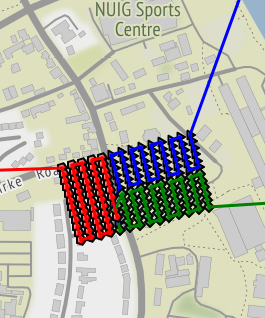
\includegraphics[width=0.65\textwidth]{Chapters/MultiAgentCoverage/Figs/RAVRoutingNUIGCropped.png}
\caption{NN heuristic encourages the creation of optimal sub-tours, which are assigned to each RAV}
\label{fig:NNPartitioning}
\end{figure}

The algorithm can be seen to be a very straightforward extension of the single agent NN algorithm. The while loop iteratively cycles through the list of RAVs and assigns the nearest non-assigned neighbor to the next RAVs partially assembled route.

Since we run this algorithm over a uniformly-spaced grid, it builds agent routes in a lawn-cutting pattern, which provides good results as long as the routes do not begin to overlap. The idea is to take the NN algorithm TSP solution and apply it exhaustively in a round-robin manner, so that each RAV is encouraged to find a non-overlapping optimal sub-tour. These non-overlapping optimal sub-tours partition the region and therefore offer a solution to the mTSP. Section 4 of \cite{Hungerlander2018TheGrids} gives an insight to how optimal solutions can be found for a uniformly spaced rectangular grid when RAVs are assumed to start in the corners of the rectangle, which provides further motivation to using Algorithm \ref{alg:NNHeuristic}. In practice non-overlapping optimal sub-tours are not found, but solutions may come close, as illustrated in Figure \ref{fig:NNPartitioning}.

%Since sometimes the solutions found by the algorithm are not always well-balanced, we propose to iteratively re-run the algorithm after a set interval in order to update the solution to ensure that no RAV is idle while others are doing work. This also ensures redundancy in the system - if a RAV stops operating, its uncompleted work will be re-assigned to the others.

%\note{Not sure if worth mentioning lower bound of cost for this algo is 1/noRAVs}
%\note{might be worth mentioning that it would be ideal to add the next grid point to whichever agent has the shortest route so far}



\subsubsection{Analysis of the NN algorithm}
%\note{The justification behind this choice of algo is a bit weak, might be worth running tests on file:///C:/Users/13383861/Downloads/graphsOR18.pdf}


The results and analysis of applying the NN heuristic algorithm to the symmetric Euclidean TSP and mTSP are well documented and we will not go into great detail repeating the results here. Instead, we refer the reader to the chapter ``The travelling salesman problem: A case study'' of \cite{Aarts:1997:LSC:549160}, written by \citeauthor{Johnson1995TheOptimization}, which provides a comparison of the NN heuristic to other heuristic algorithms. They compare solutions with the standard Held-Karp lower bound \cite{Held1962AProblems} using a standardised library of Travelling Salesman Problems, TSPLIB \cite{TSPLIB}. Rather than provide tables of results showing the performance of the NN heuristic algorithm on standard benchmark data sets such as TSPLIB, we instead focus on the results for the domain we are most interested in, which is a connected graph defined by a uniformly spaced set of grid points. We found that the algorithm performed best when the RAVs used regions that have multiple axes of symmetry. Rectangular regions in particular yield scalable, high-quality solutions, as shown in the figures in Table \ref{table:NNAlgoResultsRect}. This corresponds to the optimal performance configuration suggested in \cite{Hungerlander2018TheGrids}. We evaluated solutions both qualitatively and  quantitatively. We focused on the qualitative results of the experiments, which were designed to show that the system can partition the in the region to give a reasonably balanced amount of work to each agent for regular polygons with a number of axes of symmetry. This was a proof-of-concept, with the intention for future work to provide a more thorough analysis on performance. We found that RAV starting points are a critical factor in solution quality, which again is in line with the findings in \cite{Hungerlander2018TheGrids}. Tables \ref{table:NNAlgoResultsRect}, \ref{table:NNAlgoResultsTri} and \ref{table:NNAlgoResultsHex} %\ref{table:NNAlgoResultsIrregular} 
illustrate some of the results, with the configuration of each listed below. The experiments are intended to demonstrate practical use cases where the NN algorithm will provide qualitatively good results.

\pagebreak
\subsection{Qualitative Behaviour of the NN Algorithm With a Rectangular Grid}
We set up this experiment with the aim of showing that if the RAVs can be placed in the configuration suggested by \citeauthor{Hungerlander2018TheGrids}, they will partition the region in a close to optimal fashion \cite{Hungerlander2018TheGrids}, minimising the longest distance any one RAV needs to travel to complete its mission. We ran the experiment using 1-4 RAVs, placing them in the corners of the rectangles. This was done in an approximate fashion by manually dragging the RAVs to their starting position using the UI mentioned in Section \ref{subsec:SceneSurveyingUI}. The results in Table \ref{table:NNAlgoResultsRect} show that the amount of work done by each RAV is approximately evenly balanced. Theoretically, the minimum amount of work done by each RAV would be $\frac{1}{2}$, $\frac{1}{3}$ and $\frac{1}{4}$ of the total work done by a single RAV when using 2, 3 and 4 RAVs respectively.
\par The results show that when using 2, 3 and 4 RAVs, the solutions found by the NN algorithm were 2.701\%, 4.500\% and 17.315\% less efficient than evenly splitting up the solution for a single RAV ( $\frac{1}{2}$, $\frac{1}{3}$ and $\frac{1}{4}$ of 3576.6, respectively). This was partly due to the extra distance added from the starting positions. Note that when using 4 RAVs, there was some overlap in the routes which added a significantly higher overhead to the cost of the route in relation to that given by even splitting the solution found for a single RAV.


We used the following configuration to run the experiment:
\\Spacing between grid points: 23m in latitude, 25m in longitude.
\\Bounding rectangle coordinates: (53.2781933786, -9.0671226391), (53.2803800539, -9.067182416), (53.2804392784, -9.0611222377), (53.2782526061, -9.0610624609)
\\

\begin{table}[H]
  \centering
  \begin{tabular}{ | c | m{5cm} | }
    \hline
    Planned RAV Routes & Route Lengths (metres) \\
    \hline
    
    %single RAV
    \begin{minipage}[c][53mm][c]{.6\textwidth}
      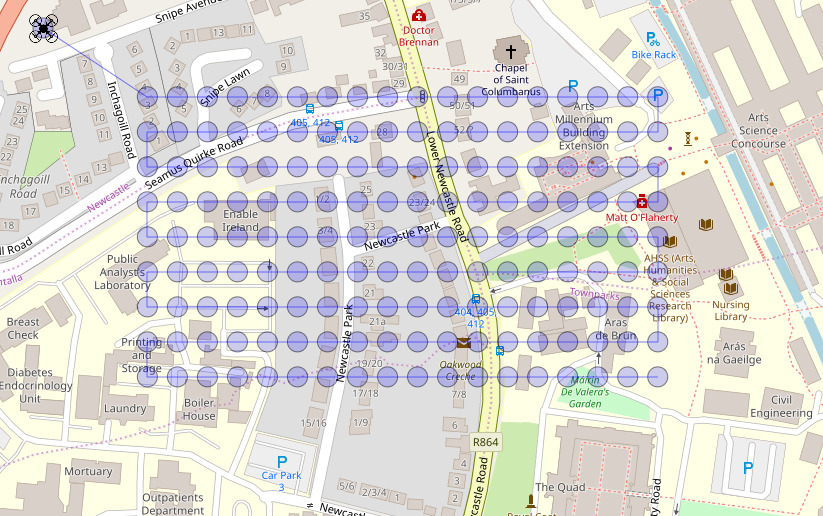
\includegraphics[width=\linewidth, height=51mm]{Chapters/MultiAgentCoverage/MultipleTravellingSalesman/Figs/Rectangle/SingleAgent.PNG}

    \end{minipage}
    &
    \begin{itemize}[leftmargin=*]
      \item[] RAV 1 (blue): 3576.6
    \end{itemize}
    \\
    \hline
    %two RAV
    \begin{minipage}[c][53mm][c]{.6\textwidth}
      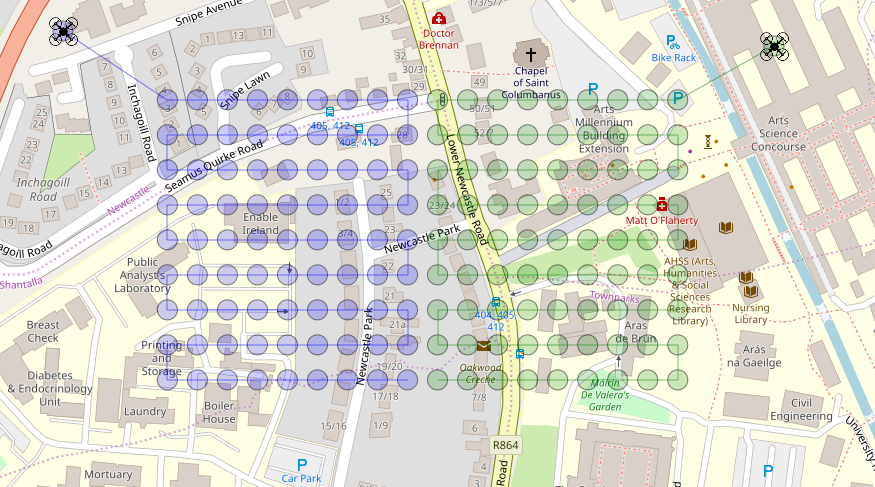
\includegraphics[width=\linewidth, height=51mm]{Chapters/MultiAgentCoverage/MultipleTravellingSalesman/Figs/Rectangle/TwoAgent.PNG}
    \end{minipage}
    &
    \begin{itemize}[leftmargin=*]
        \item[] RAV 1 (blue): 1836.3
        \item[] RAV 2 (green): 1825.8
    \end{itemize}
    \\
    \hline
    
    %three RAV
    \begin{minipage}[c][53mm][c]{.6\textwidth}
      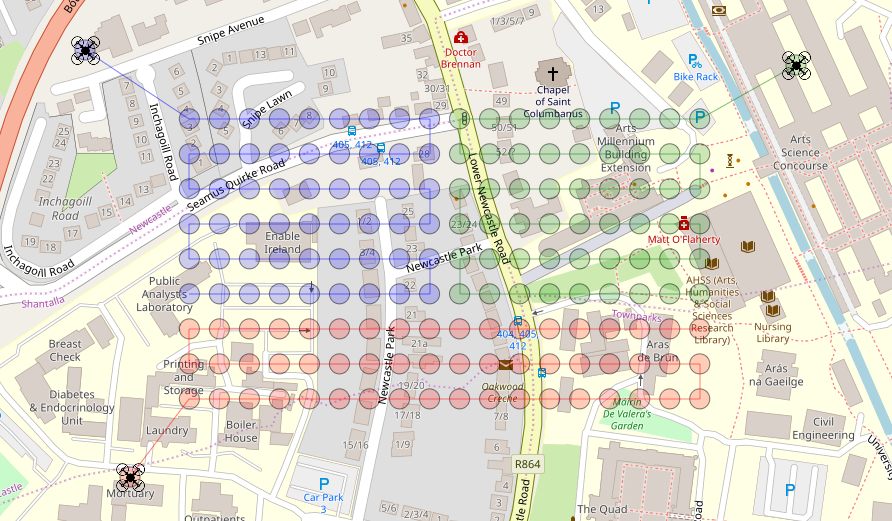
\includegraphics[width=\linewidth, height=51mm]{Chapters/MultiAgentCoverage/MultipleTravellingSalesman/Figs/Rectangle/ThreeAgent.PNG}
    \end{minipage}
    &
    \begin{itemize}[leftmargin=*]
    \item[] RAV 1 (blue): 1245.6
    \item[] RAV 2 (green): 1235.1
    \item[] RAV 3 (red): 1215.9
    \end{itemize}
    \\
    \hline
    
    %Four RAV
    \begin{minipage}[c][53mm][c]{.6\textwidth}
      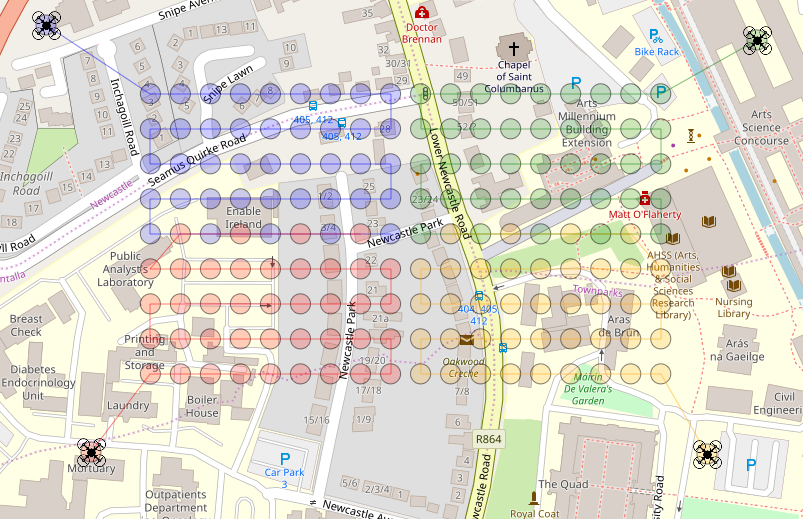
\includegraphics[width=\linewidth, height=51mm]{Chapters/MultiAgentCoverage/MultipleTravellingSalesman/Figs/Rectangle/FourAgent.PNG}
    \end{minipage}
    &
    \begin{itemize}[leftmargin=*]
    \item[] RAV 1 (blue): 1048.8
    \item[] RAV 2 (green): 1038.3
    \item[] RAV 3 (red): 994.5
    \item[] RAV 4 (yellow): 990.5
    \end{itemize}

    \\
    \hline
  \end{tabular}
  \caption{Results of applying NN algorithm to a rectangular region}\label{table:NNAlgoResultsRect}
\end{table}




\pagebreak
\subsection{Qualitative Behaviour of the NN Algorithm With a Triangular Grid}
This experiment was set up in a similar manner to the first, where the RAVs were dragged to an initial starting position that should allow the NN algorithm to take advantage of the axes of symmetry of the triangle.
The results in Table \ref{table:NNAlgoResultsTri} show that the amount of work done by each RAV is approximately evenly balanced when using two RAVs, but not three. 

The results show that when using two and three RAVs, the solutions found by the NN algorithm were 0.155\% and 36.565\% less efficient than that given by even splitting the solution for a single RAv ( $\frac{1}{2}$ and $\frac{1}{3}$ of 1940.6, respectively). This can be explained by the corresponding figures displaying the agents routes in Table \ref{table:NNAlgoResultsTri}. Clearly, the NN algorithm takes advantage of the symmetry down the center axis when two RAVs are used, but when three RAVs are used, the solution the RAV beginning at the top of the triangle skips the grid points that require a "diagonal" move, instead moving down to the closer grid point. These points are picked up by the second RAV (green) once it meets the third (red), adding a relatively large cost.

We used the following configuration to run the experiment:
\\Spacing between grid points: 23m in latitude, 25m in longitude.
\\Bounding rectangle coordinates: (53.2781933786, -9.0671226391), (53.2782526061, -9.0610624609), (53.2803800539, -9.06409255)
\\

%\\Spacing between grid points: 23m in latitude, 25m in longitude.
%\\Bounding rectangle coordinates: (53.2781933786, -9.0671226391), (53.2782526061, -9.0610624609), (53.2803800539, -9.06409255)
\begin{table}[H]
  \centering
  \begin{tabular}{ | c | m{5cm} | }
    \hline
    Planned RAV Routes & Route Lengths (metres) \\
    \hline
    
    %single RAV
    \begin{minipage}[c][57mm][c]{.6\textwidth}
      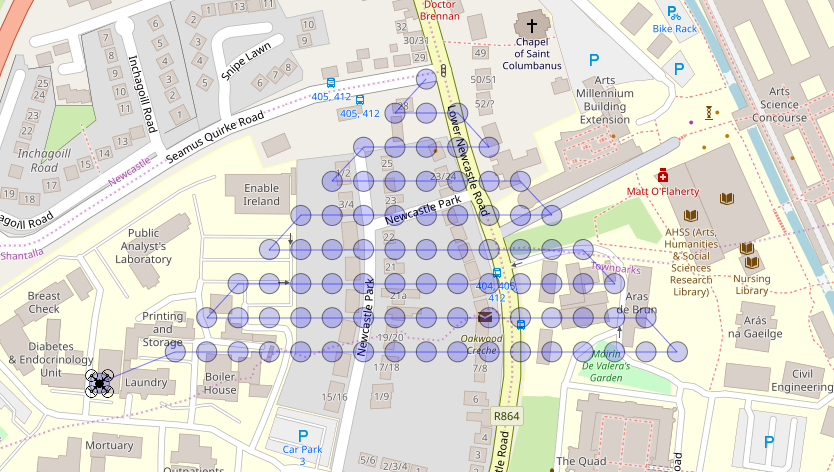
\includegraphics[width=\linewidth, height=55mm]{Chapters/MultiAgentCoverage/MultipleTravellingSalesman/Figs/Triangle/OneRAV.PNG}
    \end{minipage}
    &
    \begin{itemize}[leftmargin=*]
      \item[] RAV 1 (blue): 1940.6
    \end{itemize}
    \\
    \hline
    %two RAV
    \begin{minipage}[c][57mm][c]{.6\textwidth}
      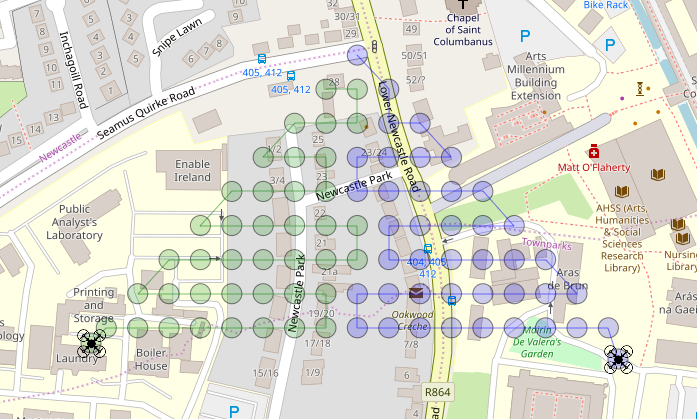
\includegraphics[width=\linewidth, height=55mm]{Chapters/MultiAgentCoverage/MultipleTravellingSalesman/Figs/Triangle/TwoRAV.PNG}
    \end{minipage}
    &
    \begin{itemize}[leftmargin=*]
        \item[] RAV 1 (blue): 971.8
        \item[] RAV 2 (green): 930.7
    \end{itemize}
    \\
    \hline
    
    %three RAV
    \begin{minipage}[c][57mm][c]{.6\textwidth}
      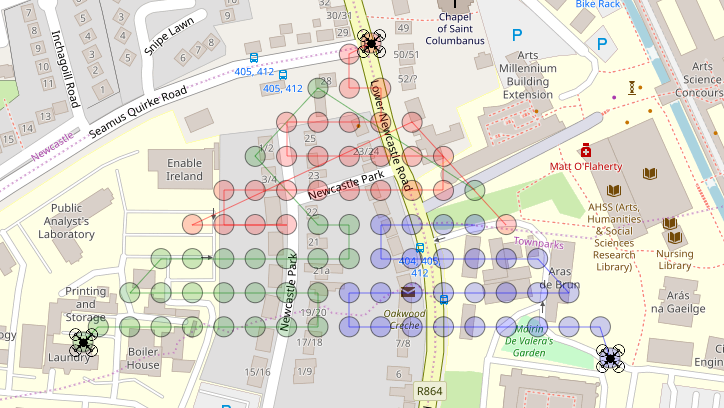
\includegraphics[width=\linewidth, height=55mm]{Chapters/MultiAgentCoverage/MultipleTravellingSalesman/Figs/Triangle/ThreeRAV.PNG}
    \end{minipage}
    &
    \begin{itemize}[leftmargin=*]
    \item[] RAV 1 (blue): 621.6
    \item[] RAV 2 (green): 812.7
    \item[] RAV 3 (red): 883.4
    \end{itemize}
    \\
    \hline
  \end{tabular}
  \caption{Results of applying NN algorithm to a triangular region}\label{table:NNAlgoResultsTri}
\end{table}


%\textbf{Hexagonal Region}
%\\Spacing between grid points: 32m in latitude, 38m in longitude.
%\\Bounding rectangle coordinates: (53.2782526061, -9.0610624609), (53.2803800539, -9.06409255), (53.2781933786, -9.0671226391), (53.27621, -9.0671226391), (53.27402, -9.06409255), (53.27615, -9.0610624609)
%\\



\pagebreak
\subsection{Qualitative Behaviour of the NN Algorithm With a Hexagonal Grid}
This experiment was again set up in a similar manner to the first, where the RAVs were dragged to starting positions that should allow the NN algorithm to take advantage of the axes of symmetry of the hexagon. In this case, we had to vary their starting locations depending on the number of RAVs used in order to encourage the generation of non-overlapping solutions. We found that the NN algorithm could find (approximately) symmetrical solutions using two or four RAVs, shown in Table \ref{table:NNAlgoResultsHex}.



The results show that when using two RAVs, the longest route is 2.191\% shorter than half the length of the route found using just one RAV. When two RAVs are used, they move horizontally to the nearest grid location, meet in the middle of the hexagon and then move back to the outer edge. Once the reach the lower third of the hexagon, they move down diagonally and then back across horizontally. This behaviour is the same when using a single RAV. The key difference is when they move to the top third of the hexagon, they exhibit the same behaviour, wheras the single agent skips some of the "diagonal" grid points, as in the case of the triangular region using three RAVs. It must go back to visit them at a relatively large cost, since the points that it missed on each from range from both the left and right sides of the upper hexagon. This can be seen in the first figure in Table \ref{table:NNAlgoResultsHex}.


When using four RAVs, the longest route was 36.565\% longer than $\frac{1}{4}$ of the length of the route found for a single RAV. This was mainly due to the slight imbalance in the number of points in the upper third and lower third of the hexagon and the middle third. There are 79 points in both the upper and lower third and 147 points in the middle third. This means that the two RAVs that sweep back and across the middle move to the upper and lower third to "help". This results in large jumps to finish of the final few grid points, visible in the third figure of table \ref{table:NNAlgoResultsHex}. 

We used the following configuration to run the experiment:
\\
Spacing between grid points: 32m in latitude, 38m in longitude.
Bounding coordinates: (53.2782526061, -9.0610624609), (53.2803800539, -9.06409255), (53.2781933786, -9.0671226391), (53.27621, -9.0671226391), (53.27402, -9.06409255), (53.27615, -9.0610624609)





\begin{table}[H]
  \centering
  \begin{tabular}{ | c | m{4.5cm} | }
    \hline
    Planned RAV Routes & Route Lengths (metres) \\
    \hline
    
    %single RAV
    \begin{minipage}[c][74mm][c]{.55\textwidth}
      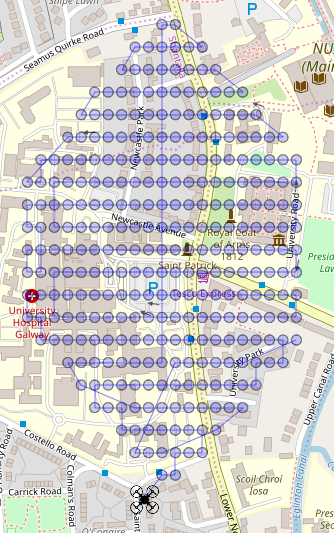
\includegraphics[width=\linewidth, height=72mm]{Chapters/MultiAgentCoverage/MultipleTravellingSalesman/Figs/Hexagon/OneRAV.PNG}
    \end{minipage}
    &
    \begin{itemize}[leftmargin=*]
      \item[] RAV 1 (blue): 7247.2
    \end{itemize}
    \\
    \hline
    %two RAV
    \begin{minipage}[c][74mm][c]{.55\textwidth}
      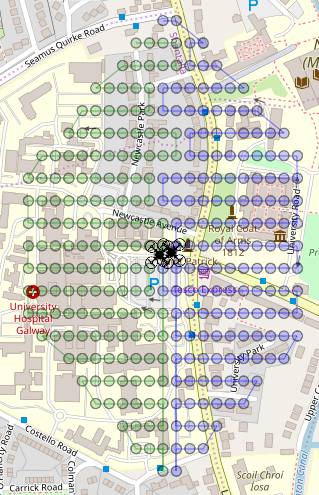
\includegraphics[width=\linewidth, height=72mm]{Chapters/MultiAgentCoverage/MultipleTravellingSalesman/Figs/Hexagon/TwoRAV.PNG}
    \end{minipage}
    &
    \begin{itemize}[leftmargin=*]
        \item[] RAV 1 (blue): 3587.4
        \item[] RAV 2 (green): 3544.2
    \end{itemize}
    \\
    \hline
    
    %three RAV
    \begin{minipage}[c][69mm][c]{.55\textwidth}
      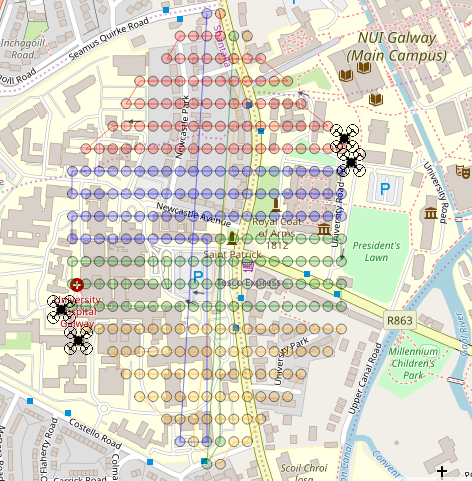
\includegraphics[width=\linewidth, height=67mm]{Chapters/MultiAgentCoverage/MultipleTravellingSalesman/Figs/Hexagon/FourRAV.PNG}
    \end{minipage}
    &
    \begin{itemize}[leftmargin=*]
    \item[] RAV 1 (blue): 2435.6
    \item[] RAV 2 (green): 1629.6
    \item[] RAV 3 (red): 2412.0
    \item[] RAV 4 (yellow): 2245.9
    \end{itemize}
    \\
    \hline
  \end{tabular}
  \caption{Results of applying NN algorithm to a hexagonal region}\label{table:NNAlgoResultsHex}
\end{table}


%\textbf{Irregular Region}
%\\Spacing between grid points: 20m in latitude, 20m in longitude.
%\\Bounding rectangle coordinates: (53.28048,-9.069021), (53.28189,-9.066017), (53.28009,-9.065223), (53.28192,-9.064128), (53.28026,-9.061725), (53.27923,-9.063957), (53.27846,-9.063721), (53.27712,-9.063721), (53.27626,-9.060159), (53.27516,-9.061124), (53.27412,-9.061425), (53.27362,-9.061425), (53.2735,-9.062562), (53.27456,-9.06327), (53.27416,-9.064794), (53.27495,-9.06754), (53.27456,-9.067841), (53.27354,-9.067605), (53.27346,-9.06857), (53.27466,-9.06872), (53.2752,-9.06827), (53.27583,-9.070008), (53.27571,-9.07093), (53.27545,-9.074385), (53.27581,-9.074149), (53.27609,-9.07445), (53.2788,-9.069986), (53.27951,-9.069793), (53.28116,-9.071081), (53.28148,-9.069686)
%\\

%\textbf{Irregular Region}
%\\Spacing between grid points: 20m in latitude, 20m in longitude.
%\\Bounding rectangle coordinates: (53.28048,-9.069021), (53.28189,-9.066017), (53.28009,-9.065223), (53.28192,-9.064128), (53.28026,-9.061725), (53.27923,-9.063957), (53.27846,-9.063721), (53.27712,-9.063721), (53.27626,-9.060159), (53.27516,-9.061124), (53.27412,-9.061425), (53.27362,-9.061425), (53.2735,-9.062562), (53.27456,-9.06327), (53.27416,-9.064794), (53.27495,-9.06754), (53.27456,-9.067841), (53.27354,-9.067605), (53.27346,-9.06857), (53.27466,-9.06872), (53.2752,-9.06827), (53.27583,-9.070008), (53.27571,-9.07093), (53.27545,-9.074385), (53.27581,-9.074149), (53.27609,-9.07445), (53.2788,-9.069986), (53.27951,-9.069793), (53.28116,-9.071081), (53.28148,-9.069686)
%\\

%\begin{table}[H]
%  \centering
%  \begin{tabular}{ | c | m{5cm} | }
%    \hline
%    Planned RAV Routes & Route Lengths (metres) \\
%    \hline
    
    %single RAV
%    \begin{minipage}[c][68mm][c]{.6\textwidth}
%      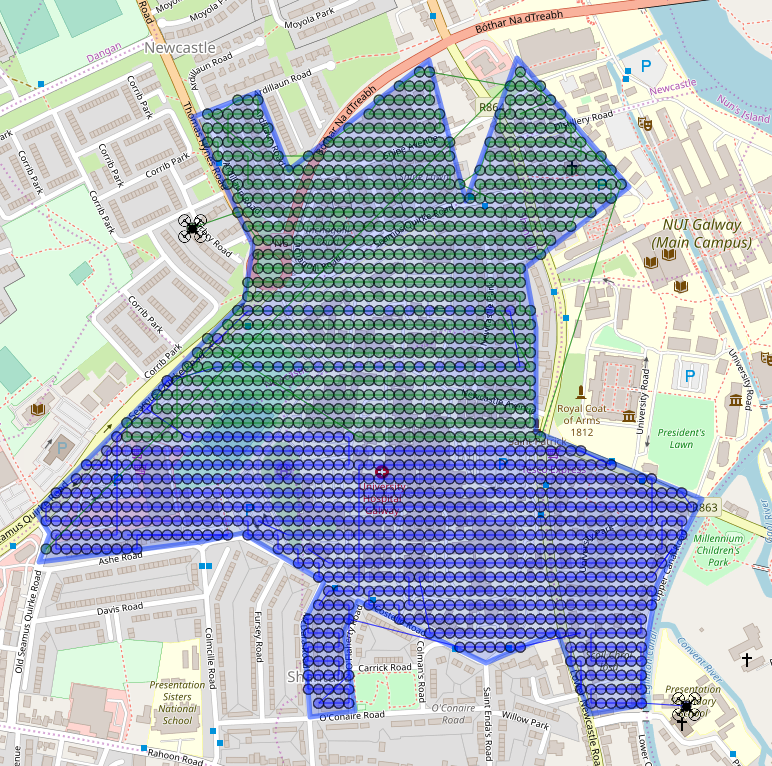
\includegraphics[width=\linewidth, height=66mm]{Chapters/MultiAgentCoverage/MultipleTravellingSalesman/Figs/IrregularRegion/TwoRAV.PNG}
%    \end{minipage}
%    &
%    \begin{itemize}[leftmargin=*]
%       \item[] RAV 1 (blue): 14268.6
%        \item[] RAV 2 (green): 13393.6
%    \end{itemize}
 %   \\
%    \hline
    %two RAV
%    \begin{minipage}[c][68mm][c]{.6\textwidth}
%      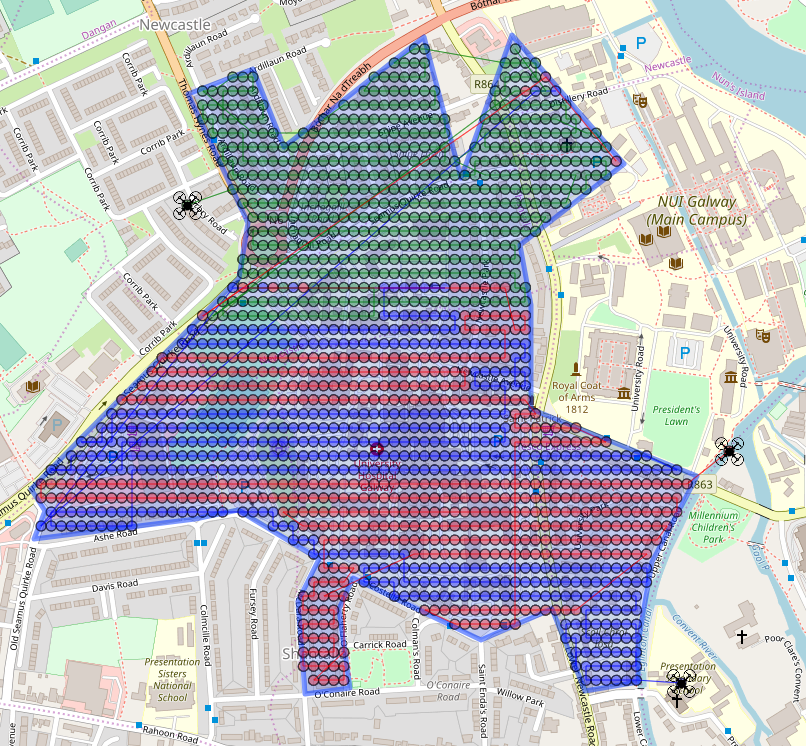
\includegraphics[width=\linewidth, height=66mm]{Chapters/MultiAgentCoverage/MultipleTravellingSalesman/Figs/IrregularRegion/ThreeRAV.PNG}
%    \end{minipage}
%    &
%    \begin{itemize}[leftmargin=*]
%        \item[] RAV 1 (blue): 8879.8
%        \item[] RAV 2 (green): 9596.4
%        \item[] RAV 3 (green): 9433.4
%    \end{itemize}
%    \\
%    \hline
    
    %three RAV
%    \begin{minipage}[c][68mm][c]{.6\textwidth}
%      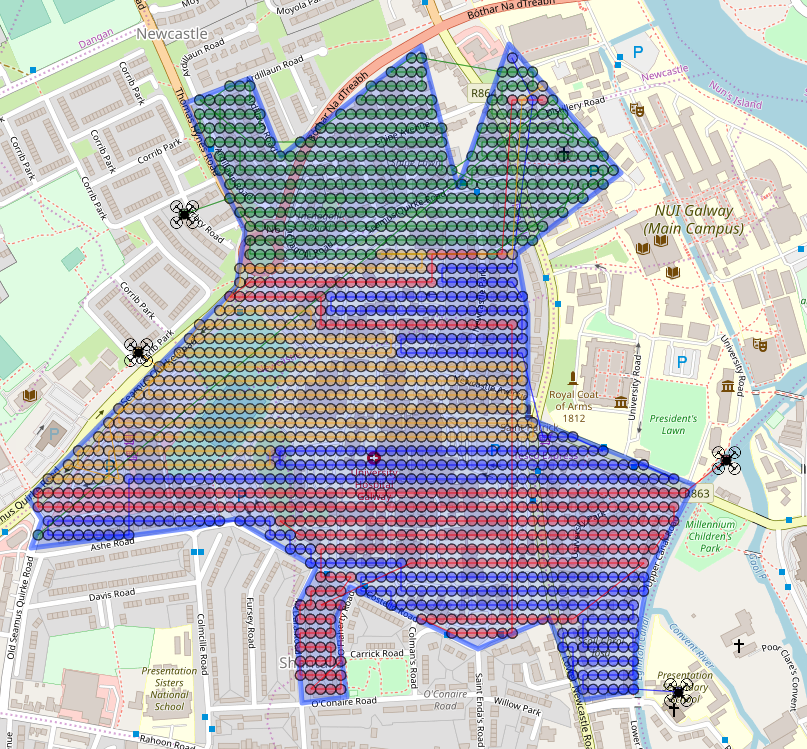
\includegraphics[width=\linewidth, height=66mm]{Chapters/MultiAgentCoverage/MultipleTravellingSalesman/Figs/IrregularRegion/FourRAVSecondAttempt.PNG}
%    \end{minipage}
%    &
%    \begin{itemize}[leftmargin=*]
%    \item[] RAV 1 (blue): 7673.2
%%    \item[] RAV 2 (green): 6354.0
 %   \item[] RAV 3 (red): 6860.6
%    \item[] RAV 4 (yellow): 6368.8
%    \end{itemize}
%    \\
%    \hline
%  \end{tabular}
%  \caption{Results of applying NN algorithm to an irregular region}\label{table:NNAlgoResultsIrregular}
%\end{table}
%\pagebreak



































%\subsubsection{Proof of Lower Bound of Nearest Neighbor Solution}
%Let O be a tour that is an optimal solution to the Travelling Salesperson Problem (TSP) for  a graph G(V, E), where E $\subseteq$ V $\times$ V, with a cost function c$(p_i, p_j)$ defined for all $(p_i, p_j)$ $\in$ E and an induced cost function 
%C($T$) = $\sum\limits_{(p_i, p_j)\in }$C$(p_i, p_j)$ defined for any tour $T$ of G.
%The optimal tour O is an ordered tuple (($p_i, p_j$), ($p_j, p_k$),..., ($p_m, p_n$)) $\subseteq$ E which satisfies:
%\[
%Cost(O) =  \min_{e \subseteq E}\sum_{(p_i, p_j) \in e} c(p_i, p_j) 
%\]
%with the constraint that each $p_i \in$ V must be visited exactly once. This means that O is a Hamiltonian tour of G of minimal cost. 
%\\
%For any partition ($T_1, T_2, ..., T_m$) of an arbitrary tour T', we find:

%\[\text{Cost}(T')=\sum\limits_{k=1}^{m}\sum\limits_{(p_i, p_j)\in T_k} \text{cost}(p_i, p_j) \leq m \times \max_{T_k \in T}
%\sum\limits_{(p_i, p_j)\in T_k}c(p_i, p_j) = 
%m \times \max_{T_k \in T} \text{Cost}(T_k)
%\]

%\noindent Since Cost(O) $\leq$ Cost(T'), for the partition determined by any solution to the TSP, we find that for any solution S to mTSP consisting of the partition ($S_1, S_2, ...,S_m$) for each of the m agents:\\

%\[
%Cost(T)
%\leq Cost(S) \leq  m \times
%\max_{S_k \in S}
%\sum\limits_{(p_i, p_j)\in S_k}C(p_i, p_j)) = Cost of MTS solution, S.
%\]
%This means we can use a solution of the standard Traveling Salesperson problem as a lower bound for comparison with Algorithm \ref{alg:agentRoutesEdited}. For example, the Held-Karp algorithm gives a well-known lower bound when dealing with a metric space \cite{VALENZUELA1997157}.

%We explored a number of solutions to this 

